\begin{figure}[H]
    \centering
    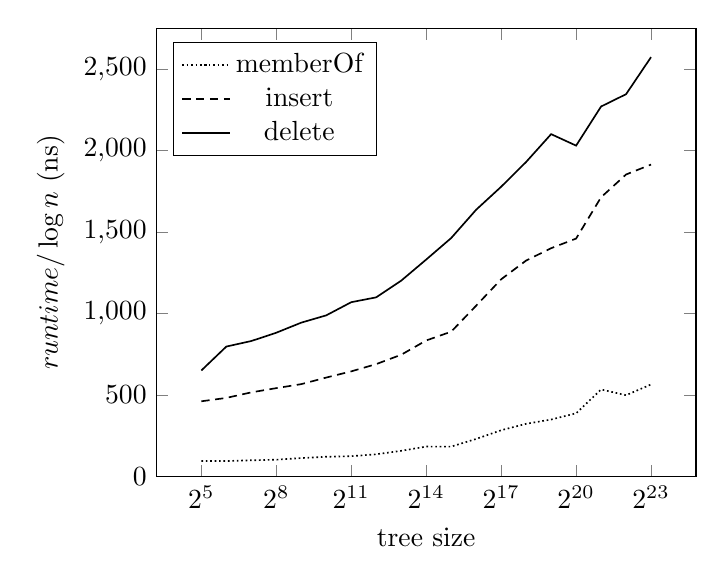
\begin{tikzpicture}
        \begin{axis}[
            xlabel=tree size,
            ylabel=$\text{runtime}/\log{n}$ (ns),
            legend pos=north west,
            ymin=0, ymax=2750,
            xtick={2^5, 2^8, 2^11, 2^14, 2^17, 2^20, 2^23},
            xmode=log,
            log basis x=2
            ]
            \addplot[densely dotted, line width=0.6pt] coordinates {
                (2^5, 95.61019589229326)
                (2^6, 95.16579057969723)
                (2^7, 99.73801239024621)
                (2^8, 103.33333333333333)
                (2^9, 113.56735564286232)
                (2^10, 121.31508825258442)
                (2^11, 124.87600496932754)
                (2^12, 136.68204336905362)
                (2^13, 157.81908218555472)
                (2^14, 183.8546745260355)
                (2^15, 183.77786181344752)
                (2^16, 230.75)
                (2^17, 284.0392793992604)
                (2^18, 323.5070174004093)
                (2^19, 349.81764526282444)
                (2^20, 388.0212634689161)
                (2^21, 534.1144034430516)
                (2^22, 498.94250888410534)
                (2^23, 565.0414484933796)
            };
            \addlegendentry{memberOf}
            \addplot[densely dashed, line width=0.6pt] coordinates {
                (2^5, 461.6852702546774)
                (2^6, 482.4054506214734)
                (2^7, 516.5004213066321)
                (2^8, 542.3333333333334)
                (2^9, 566.8903835839544)
                (2^10, 607.17750125425)
                (2^11, 645.1926923415256)
                (2^12, 689.8259045952441)
                (2^13, 747.208496991539)
                (2^14, 834.7002223482011)
                (2^15, 888.6862621396793)
                (2^16, 1048.25)
                (2^17, 1210.0415813167458)
                (2^18, 1324.9638777889263)
                (2^19, 1400.6830345314977)
                (2^20, 1459.7651468249205)
                (2^21, 1713.2186214445712)
                (2^22, 1852.926719509826)
                (2^23, 1913.7573629136098)
            };
            \addlegendentry{insert}
            \addplot[solid, line width=0.6pt] coordinates {
                (2^5, 650.7522792488969)
                (2^6, 797.3036357103903)
                (2^7, 831.3875747101238)
                (2^8, 882.3333333333334)
                (2^9, 944.1863762196859)
                (2^10, 988.8835357561782)
                (2^11, 1069.539857376185)
                (2^12, 1099.3141488111025)
                (2^13, 1201.7490727382908)
                (2^14, 1331.107843568497)
                (2^15, 1463.0560698129052)
                (2^16, 1636.75)
                (2^17, 1777.63083903103)
                (2^18, 1929.770918473754)
                (2^19, 2100.3183250571465)
                (2^20, 2029.8810640505671)
                (2^21, 2269.872379508621)
                (2^22, 2345.3661574916214)
                (2^23, 2572.7513214264286)
            };
            \addlegendentry{delete}
        \end{axis}
    \end{tikzpicture}
    \caption{Plot of the median $\textsf{runtime}/\log{n}$ for \code{memberOf}, \code{insert} and \code{delete}}
    \label{memberOf-insert-delete-median-logn-plot}
    \end{figure}